\begin{enumerate}[label=\thechapter.\arabic*,ref=\thechapter.\theenumi]

\item Consider the differential equation $\frac{d^2y}{dx^2}-2\frac{dy}{dx}+y=0$. The boundary conditions are $y=0$ and $\frac{dy}{dx}=1$ at $x=0$. Then the value of $y$ at $x=\frac{1}{2}$ \hfill (GATE AE 2022)\\
\solution
\input{2022/AE/37/ae_37.tex}
\pagebreak

\item  A process described by the transfer function
\begin{align}
    G_p(s) = \frac{\brak{10s+1}}{\brak{5s+1}} \nonumber
\end{align}
is forced by a unit step input at time $t = 0$. The output value immediately after the unit step input (at $t = 0^+$) is ? \hfill(Gate 2022 CH 34)\\
\solution
\iffalse
\documentclass[journal,12pt,twocolumn]{IEEEtran}
\usepackage{cite}
\usepackage{amsmath,amssymb,amsfonts,amsthm}
\usepackage{algorithmic}
\usepackage{graphicx}
\usepackage{textcomp}
\usepackage{xcolor}
\usepackage{txfonts}
\usepackage{listings}
\usepackage{enumitem}
\usepackage{mathtools}
\usepackage{gensymb}
\usepackage{comment}
\usepackage[breaklinks=true]{hyperref}
\usepackage{tkz-euclide}
\usepackage{listings}
\usepackage{gvv}
\def\inputGnumericTable{}
\usepackage[latin1]{inputenc}
\usepackage{color}
\usepackage{array}
\usepackage{longtable}
\usepackage{calc}
\usepackage{multirow}
\usepackage{hhline}
\usepackage{ifthen}
\usepackage{lscape}
\usepackage{caption}

\newtheorem{theorem}{Theorem}[section]
\newtheorem{problem}{Problem}
\newtheorem{proposition}{Proposition}[section]
\newtheorem{lemma}{Lemma}[section]
\newtheorem{corollary}[theorem]{Corollary}
\newtheorem{example}{Example}[section]
\newtheorem{definition}[problem]{Definition}
\newcommand{\BEQA}{\begin{eqnarray}}
\newcommand{\EEQA}{\end{eqnarray}}
\newcommand{\define}{\stackrel{\triangle}{=}}
\theoremstyle{remark}
\newtheorem{rem}{Remark}
\begin{document}

\bibliographystyle{IEEEtran}
\vspace{3cm}

\title{GATE: CH - 34.2022}
\author{EE23BTECH11010 - Venkatesh D Bandawar $^{*}$% <-this % stops a space
}
\maketitle
% \newpage
\bigskip

% \renewcommand{\thefigure}{\theenumi}
% \renewcommand{\thetable}{\theenumi}

\textbf{Question:} A process described by the transfer function
\begin{align}
    G_p(s) = \frac{\brak{10s+1}}{\brak{5s+1}} \nonumber
\end{align}
is forced by a unit step input at time $t = 0$. The output value immediately after the unit step input (at $t = 0^+$) is ? \hfill(Gate 2022 CH 34)\\
\solution
\fi
\begin{table}[!h] 
\centering
\begin{tabular}{|c|c|}
\hline
     \textbf{Parameters}&\textbf{Description}  \\
     \hline
     $X(s)$ & Laplace transform of $x(t)$ \\
     \hline
     $Y(s)$ & Laplace transform of $y(t)$ \\
     \hline
     $G_p(s) = \frac{Y(s)}{X(s)}$ & Transfer function\\
     \hline
     $x(t) = u(t)$ & unit step function\\
     \hline
\end{tabular}

\caption{Given parameters}
\label{given parameters list.gate.2022.ch.34}
\end{table}
\begin{align}
    G_p(s) = \frac{Y(s)}{X(s)} &= \frac{\brak{10s+1}}{\brak{5s+1}}\\
    u(t) \system{\mathcal{L}} \frac{1}{s} \label{laplace transform of unit function 2022.ch.34}
\end{align}
From equation \eqref{laplace transform of unit function 2022.ch.34}:
\begin{align}
    Y(s) &= \frac{\brak{10s+1}}{s\brak{5s+1}}\\
    &= \frac{1}{s} + \frac{5}{5s+1}
\end{align}
Taking inverse laplace transformation, 
\begin{align}
    \frac{1}{s} &\mathrel{\substack{\mathcal{L}^{-1}\\\longleftrightarrow}} u(t)\\
    \frac{1}{s-c} &\mathrel{\substack{\mathcal{L}^{-1}\\\longleftrightarrow}} e^{ct} u(t)
\end{align}
\begin{align}
    y(t) &= \brak{1 + e^{\frac{-t}{5}}}u(t)\\
    y(0^+) &= 2
\end{align}

\begin{figure}[!h] 
    \centering
    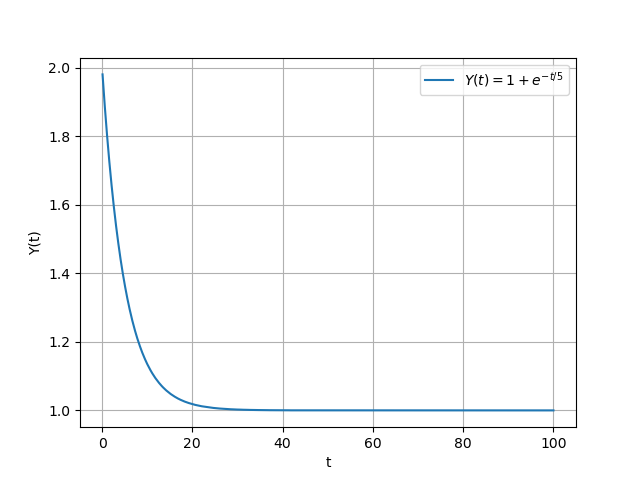
\includegraphics[width=\columnwidth]{2022/CH/34/figs/Graph_of_y(t).png}
    \caption{Graph of y(t)}
    \label{fig:Graph1_gate_CE_30}
    \end{figure}


\pagebreak
\item The transfer function of a real system $H(S)$ is given as:
\begin{align}
    H(s) = \frac{As + B}{s^2 + Cs + D}\nonumber
\end{align}
where $A, B, C$ and $D$ are positive constants. This system cannot operate as
\begin{enumerate}[label={(\Alph*)}]
    \item Low pass filter
    \item High pass filter
    \item Band pass filter
    \item An Integrator
\end{enumerate}\hfill(GATE EE 11 2022)

\solution
 \iffalse
\let\negmedspace\undefined
\let\negthickspace\undefined
\documentclass[journal,12pt,twocolumn]{IEEEtran}
\usepackage{cite}
\usepackage{amsmath,amssymb,amsfonts,amsthm}
\usepackage{algorithmic}
\usepackage{graphicx}
\usepackage{textcomp}
\usepackage{xcolor}
\usepackage{txfonts}
\usepackage{listings}
\usepackage{enumitem}
\usepackage{mathtools}
\usepackage{gensymb}
\usepackage{comment}
\usepackage[breaklinks=true]{hyperref}
\usepackage{tkz-euclide} 
\usepackage{listings}
\usepackage{gvv} 
\usepackage{caption}
\def\inputGnumericTable{}                   

%\usepackage[latin1]{inputenc}                                
\usepackage{color}                                            
\usepackage{array}                                            
\usepackage{longtable}                                       
\usepackage{calc}                                             
\usepackage{multirow}                                         
\usepackage{hhline}                                           
\usepackage{ifthen}                                           
\usepackage{lscape}
\usepackage{tikz}
\newtheorem{theorem}{Theorem}[section]
\newtheorem{problem}{Problem}
\newtheorem{proposition}{Proposition}[section]
\newtheorem{lemma}{Lemma}[section]
\newtheorem{corollary}[theorem]{Corollary}
\newtheorem{example}{Example}[section]
\newtheorem{definition}[problem]{Definition}
\newcommand{\BEQA}{\begin{eqnarray}}
\newcommand{\EEQA}{\end{eqnarray}}
\newcommand{\define}{\stackrel{\triangle}{=}}
\theoremstyle{remark}
\newtheorem{rem}{Remark}

\begin{document}

\bibliographystyle{IEEEtran}
\vspace{3cm}

\title{GATE: EE - 11.2022}
\author{EE23BTECH11013 - Avyaaz$^{*}$% <-this % stops a space 
}
\maketitle
\newpage
\bigskip

\renewcommand{\thefigure}{\arabic{figure}}
\renewcommand{\thetable}{\arabic{table}}

\large\textbf{\textsl{Question:}}
The transfer function of a real system $H(S)$ is given as:
\begin{align}
    H(s) = \frac{As + B}{s^2 + Cs + D}\nonumber
\end{align}
where $A, B, C$ and $D$ are positive constants. This system cannot operate as
\begin{enumerate}[label={(\Alph*)}]
    \item Low pass filter
    \item High pass filter
    \item Band pass filter
    \item An Integrator
\end{enumerate}\hfill(GATE EE 11 2022) \\
\solution
\fi
The transfer function $H(s)$ is given by: 
\begin{align}
    H(s) = \frac{As + B}{s^2 + Cs + D}\label{eq:given.EE.11.2022}
\end{align}
Put $s = j\omega$ in \eqref{eq:given.EE.11.2022}:
\begin{align}
    H(j\omega) = \frac{A(j\omega) + B}{(j\omega)^2 + C(j\omega) + D} \\
    |H(j\omega)| = \frac{\sqrt{(A\omega)^2 + B^2}}{\sqrt{(D - \omega^2)^2 + (\omega C)^2}}\label{eq:magnitude.EE.11.2022}
\end{align}


\begin{table}[htbp]
\setlength{\extrarowheight}{4pt}
\setlength{\tabcolsep}{3pt}
\centering
\begin{tabular}{|c|c|}
\hline
\textbf{Parameter} & \textbf{Description}\\
\hline 
Low Pass Filter & The gain should be finite at low frequency  \\
\hline
High Pass Filter &The gain should be finite at high frequency \\
\hline
Band Pass Filter& Finite gain over frequency band \\
\hline
Integrator & Transfer function should have at least\\& one pole at origin \\
\hline
\end{tabular}

\caption{Conditions}
\label{tab:inputs.EE.11.2022}
\end{table}
% \item \noindent From \tabref{tab:inputs.EE.11.2022} and equation \eqref{eq:magnitude.EE.11.2022}:
\begin{enumerate}[label={\alph*)}]
    \item Low Pass Filter:
    
  At low frequency $(\omega = 0 )$:
 \begin{align}
     |H(\omega = 0)| = \frac{B}{D}\label{eq:lowpass.EE.11.2022}
 \end{align}
$\therefore$ H(s) can operate as Low pass filter.

\item High Pass Filter:

% From \tabref{tab:inputs.EE.11.2022} and equation \eqref{eq:magnitude.EE.11.2022}:

At high frequency $(\omega = \infty )$:
 \begin{align}
     |H(\omega = \infty)| = 0 \label{eq:highpass.EE.11.2022}
 \end{align}
 % From \tabref{tab:inputs.EE.11.2022}:
 
$\therefore$ $H(s)$ cannot operate as High pass filter.
\item Band Pass Filter:

 Assuming B is a very less positive valued constant as compared to others:
\begin{align}
        |H(j\omega)| = \frac{(A\omega)}{\sqrt{(D - \omega^2)^2 + (\omega C)^2}}\\
   \implies      |H(\omega = 0)| = 0 \text{ and }  |H(\omega = \infty)| = 0 \label{eq:bandpass.EE.11.2022}
\end{align}

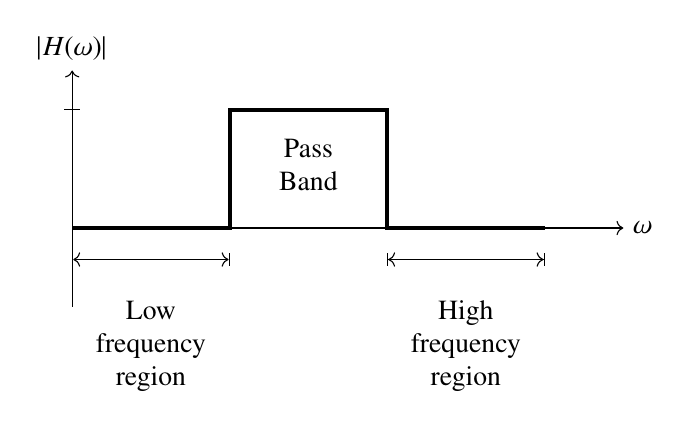
\begin{tikzpicture}
  
    \draw[->] (0,0) -- (7,0) node[right] {$\omega$};
   
    \draw[->] (0,-1) -- (0,2) node[above] {$|H(\omega)|$};
  
    \draw[line width=1.5pt]  (0,0) -- (2,0) -- (2,1.5) -- (4,1.5) -- (4,0) --(6,0);
    \draw[-]{(0,1.5)};
      \draw (-0.1,1.5) -- (0.1,1.5);
         \draw[|<->|]{(0,-0.4) -- (2,-0.4)};
    \node[align=center] at (1,-1.5) {Low \\frequency\\ region};
         \draw[| <-> |]{(4,-0.4) -- (6,-0.4)};
    \node[align=center] at (5,-1.5) {High \\frequency\\ region};
    \node[align=center] at (3,0.8) {Pass\\Band};

\end{tikzpicture}
$\because$ $H(s)$ passes frequency between low and high frequencies.

$\therefore$ $H(s)$ can operate as a band pass filter.
\item Integrator:

At very high value of frequency$(\omega\mkern-4mu \rightarrow\mkern-6mu\infty)$:
\begin{align}
    H(s) \approx \frac{As}{s^2} \approx \frac{A}{s}\label{eq:integrator.EE.11.2022}
\end{align}
From \tabref{tab:inputs.EE.11.2022}:

$\therefore$ $H(s)$ can operate as an Integrator.
\end{enumerate}
% From equations \eqref{eq:lowpass.EE.11.2022},\eqref{eq:highpass.EE.11.2022},\eqref{eq:bandpass.EE.11.2022} and \eqref{eq:integrator.EE.11.2022}:

% The Transfer function $H(s)$ cannot be operated as a High pass filter.
% \begin{figure}[htbp]
%     \centering
%     \includegraphics[width = \columnwidth]{}
%   \caption{}
%     \label{fig:graph1}
% \end{figure}

% \bibliographystyle{IEEEtran}
%\end{document}

\pagebreak

\item In a circuit, there is a series connection of an ideal resistor and an ideal capacitor.
The conduction current (in Amperes) through the resistor is $2\sin\brak{t + \frac{\pi}{2}}$. The displacement current (in Amperes) through the capacitor is \rule{1cm}{0.15mm}.\\ 
\begin{enumerate}[label=(\Alph*)]
    \item $2\sin\brak{t}$
    \item $2\sin\brak{t+\pi}$
    \item $2\sin\brak{t +\frac{\pi}{2}}$
    \item $0$
\end{enumerate}
\hfill(GATE 2022 EC 24)\\
\solution
\iffalse
\documentclass[journal,12pt,twocolumn]{IEEEtran}
\usepackage{amsmath,amssymb,amsfonts,amsthm}
\usepackage{txfonts}
\usepackage{tkz-euclide}
\usepackage{listings}
\usepackage{gvv}
\usepackage[latin1]{inputenc}
\usepackage{adjustbox}
\usepackage{array}
\usepackage{tabularx}
\usepackage{enumitem}
\usepackage{pgf}
\usepackage{lmodern}
\usepackage{circuitikz}
\usepackage{tikz}
\usepackage{graphicx}


\begin{document}
\bibliographystyle{IEEEtran}

\vspace{3cm}

\title{}
\author{EE23BTECH11054 -  Sai Krishna Shanigarapu$^{*}$
}
\maketitle
\newpage
\bigskip

% \renewcommand{\thefigure}{\theenumi}
% \renewcommand{\thetable}{\theenumi}

\section*{Gate EC 2022}
54. \hspace{2pt}In a circuit, there is a series connection of an ideal resistor and an ideal capacitor.
The conduction current (in Amperes) through the resistor is $2\sin\brak{t + \frac{\pi}{2}}$. The displacement current (in Amperes) through the capacitor is \rule{1cm}{0.15mm}.\\ 
\begin{enumerate}[label=(\Alph*)]
    \item $2\sin\brak{t}$
    \item $2\sin\brak{t+\pi}$
    \item $2\sin\brak{t +\frac{\pi}{2}}$
    \item $0$
\end{enumerate}
\hfill(GATE EC 2022)

\solution
\fi
\begin{table}[ht]
       \setlength{\arrayrulewidth}{0.3mm}
\setlength{\tabcolsep}{20pt}
\renewcommand{\arraystretch}{1.5}

\begin{tabular}{|c|c|c|}
\hline
Parameter& Description & Value\\
\hline
$I_c$ & Conduction Current & $2\sin\brak{t + \frac{\pi}{2}}$\\
\hline
%$I_d$ & Displacement current & ?\\
%\hline
$A$ & Cross-sectional area & \\
\hline
\end{tabular}

    \caption{Parameters}
    \label{tab:tab_gate_ec_2022_24_1}
\end{table}


\begin{table}[ht]
       \setlength{\arrayrulewidth}{0.3mm}
\setlength{\tabcolsep}{20pt}
\renewcommand{\arraystretch}{1.5}

\begin{tabular}{|c|c|c|}
\hline
Parameter & Description & Formula\\
\hline
$Q$ & Charge & $\int I_c\, dt$\\
\hline
$D$ & Electric Displacement & $\frac{Q}{A}$\\ 
\hline
$J_D$ & Displacement current density & $\frac{\partial D}{\partial t}$\\
\hline
$I_D$ & Displacement current & $J_D\text{ x }A$\\
\hline




\end{tabular}

    \caption{Formulae}
    \label{tab:tab_gate_ec_2022_24_2}
\end{table}

\begin{table}[ht]
       \setlength{\arrayrulewidth}{0.3mm}
\setlength{\tabcolsep}{20pt}
\renewcommand{\arraystretch}{1.5}



\begin{tabular}{|c|c|}
\hline

S Domain & Time Domain\\
\hline
$\frac{1}{s}$ & $u\brak{t}$\\
\hline
$\frac{-s}{a^2+s^2}$ & $-\cos\brak{at}$\\
\hline
$\frac{a}{a^2+s^2}$ & $\sin\brak{at}$\\
\hline
$\frac{1}{s+a}$ & $e^{-at}$\\
\hline

\end{tabular}


    \caption{Laplace transforms}
    \label{tab:tab_gate_ec_2022_24_3}
\end{table}

\begin{align}
    \mathcal{L}\sbrak{\int f\brak{t}\, dt} &= \int_{0}^{\infty}\sbrak{\int f\brak{t}\, dt}e^{-st}\, dt\\
    &= \int_{0}^{\infty}u\, dv \quad \text{where}\begin{cases}
  u =\int f\brak{t}dt \\
  dv  =e^{-st}dt
\end{cases}\\
&= uv - v\int du\\
&= \frac{1}{s}\int f\brak{t}dt|_0 + \frac{1}{s}\int_{0}^{\infty}f\brak{t}e^{-st}dt\\
&\implies \frac{1}{s}\int f\brak{t}dt|_0 + \frac{1}{s}F\brak{s} \label{eq:eq_gate_ec_2022_24_1}
\end{align}


\begin{figure}[ht]
  \centering
      \begin{circuitikz}[american]
\draw (0,3) to [short,*-, i=$i_c$] (1,3) to [R=$R$] (4,3);
\draw (0,0) to [short, *-] (4,0);
\draw (4,3) to [short, i=$i_d$] (4,2.5) to [C=$C$] (4,0);
\end{circuitikz}
  \caption{Circuit 1}
\end{figure}

From Table \ref{tab:tab_gate_ec_2022_24_2}, Table \ref{tab:tab_gate_ec_2022_24_3} and eq (\ref{eq:eq_gate_ec_2022_24_1})
\begin{align}
    I_c\brak{s} &= \frac{2s}{s^2 + 1}\\
    Q_c\brak{s} &= \frac{2}{s\brak{s^2 + 1}}\\
    D\brak{s} &= \frac{1}{A}\brak{\frac{2}{s\brak{s^2 + 1}}}\\
    J_D\brak{s} &= \frac{2}{A}\brak{\frac{1}{s^2 + 1}}\\
    I_D\brak{s} &= \frac{2}{s^2 + 1}\\
    \implies I_D &= 2\sin{t}
\end{align}


\begin{figure}[ht]
  \centering
      \begin{tikzpicture}

        \draw[->] (-0.5,0) -- (4.5,0) node[right]{$E_{\text{ref}}$};
        \draw[->] (0,-0.5) -- (0,4.5) node[above]{$J_d$};
        

        \draw (0,0) -- (4,4);
        

        \draw[dashed] (4,0) -- (4,4);
        \node[right] at (4,4) {$\overline{J}$};
        \draw[dotted] (4,4) -- (4,0) node[below]{$J_c$};

        \draw[dashed] (0,4) -- (4,4);
        \draw[dotted] (4,4) -- (0,4) node[left]{$J_d$};
        

        \draw[->] (0.5,0) arc (0:90:0.5);
        \node[right] at (0.5,0.3) {$\frac{\pi}{2}$};
\end{tikzpicture}


  \caption{Phasor plot}
  \label{fig:fig_gate_ec_2022_24_1}
\end{figure}

From figure \ref{fig:fig_gate_ec_2022_24_1}, phase of $I_d$ is $\frac{\pi}{2}$

\begin{align}
    \therefore I_d = 2\sin\brak{t + \frac{\pi}{2}}
\end{align}
$\therefore$ (C) is correct.


\begin{figure}[ht]
    \centering
    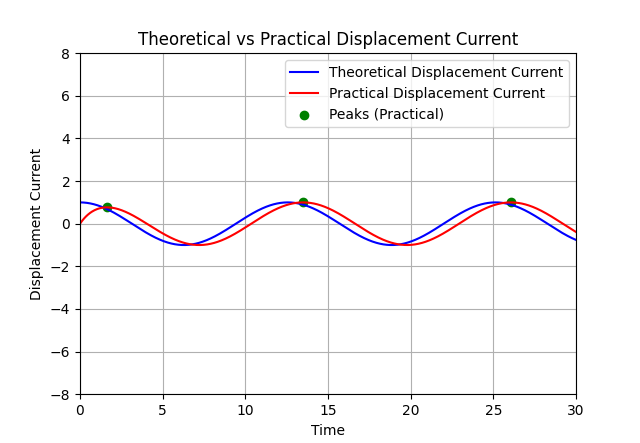
\includegraphics[width=\columnwidth]{2022/EC/24/figs/Figure_2.png}
    \caption{Thoritical vs Practical simulation}
    \label{fig:fig_gate_ec_2022_24_2}
\end{figure}

\begin{figure}[ht]
    \centering
    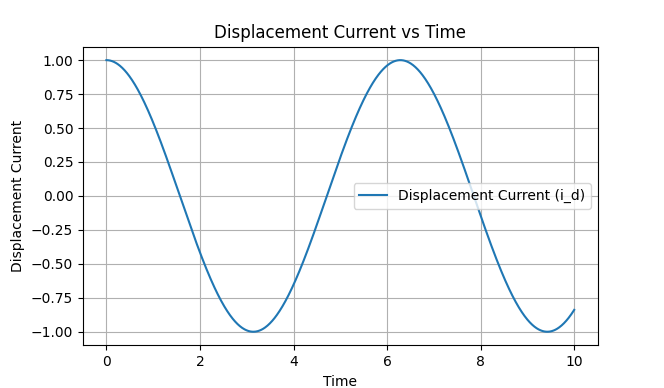
\includegraphics[width=\columnwidth]{2022/EC/24/figs/Figure_4.png}
    \caption{Displacement current}
    \label{fig:fig_gate_ec_2022_24_3}
\end{figure}



%\end{document}

\newpage

\item Given, $y=f\brak{x}$; $\frac{d^2y}{dx2}+4y=0; y\brak{0}=0; \frac{dy}{dx}\brak{0}=1$. The problem is a/an \\
\begin{enumerate}[label=(\alph*)]
    \item initial value problem having soluition $y=x$
    \item boundary value problem having soluition $y=x$
    \item initial value problem having soluition $y=\frac{1}{2}\sin 2x$
    \item boundary value problem having soluition {$y=\frac{1}{2}\sin 2x$}
\end{enumerate} \hfill(GATE 2022 ES)    \\
\solution
\iffalse
\let\negmedspace\undefined
\let\negthickspace\undefined
\documentclass[journal,12pt,twocolumn]{IEEEtran}
\usepackage{cite}
\usepackage{amsmath,amssymb,amsfonts,amsthm}
\usepackage{algorithmic}
\usepackage{graphicx}
\usepackage{textcomp}
\usepackage{xcolor}
\usepackage{txfonts}
\usepackage{listings}
\usepackage{enumitem}
\usepackage{mathtools}
\usepackage{gensymb}
\usepackage{comment}
\usepackage[breaklinks=true]{hyperref}
\usepackage{tkz-euclide} 
\usepackage{listings}
\usepackage{gvv}                                        
\def\inputGnumericTable{}                                 
\usepackage[latin1]{inputenc}                                
\usepackage{color}                                            
\usepackage{array}                                            
\usepackage{longtable}                                       
\usepackage{calc}                                             
\usepackage{multirow}                                         
\usepackage{hhline}                                           
\usepackage{ifthen}                                           
\usepackage{lscape}

\newtheorem{theorem}{Theorem}[section]
\newtheorem{problem}{Problem}
\newtheorem{proposition}{Proposition}[section]
\newtheorem{lemma}{Lemma}[section]
\newtheorem{corollary}[theorem]{Corollary}
\newtheorem{example}{Example}[section]
\newtheorem{definition}[problem]{Definition}
\newcommand{\BEQA}{\begin{eqnarray}}
\newcommand{\EEQA}{\end{eqnarray}}
\newcommand{\define}{\stackrel{\triangle}{=}}
\theoremstyle{remark}
\newtheorem{rem}{Remark}
\begin{document}
\parindent 0px
\bibliographystyle{IEEEtran}
\title{GATE: ES - 36.2022}
\author{EE22BTECH11219 - Rada Sai Sujan$^{}$% <-this % stops a space
}
\maketitle
\newpage
\bigskip
\section*{Question}
Given, $y=f\brak{x}$; $\frac{d^2y}{dx2}+4y=0; y\brak{0}=0; \frac{dy}{dx}\brak{0}=1$. The problem is a/an \\
\begin{enumerate}[label=(\alph*)]
    \item initial value problem having soluition $y=x$
    \item boundary value problem having soluition $y=x$
    \item initial value problem having soluition $y=\frac{1}{2}\sin 2x$
    \item boundary value problem having soluition {$y=\frac{1}{2}\sin 2x$}
\end{enumerate} \hfill(GATE 2022 ES)    \\
\solution
\fi

The above equation can be written as,
\begin{align}
    y^{\prime\prime}\brak{t}+4y\brak{t}=0
\end{align}
Using the Laplace transformation pairs,
\begin{align}
    y^{\prime\prime}\brak{t} &\overset{\mathcal{L}}{ \longleftrightarrow} s^2Y\brak{s}-sy\brak{0}-y^{\prime}\brak{0}    \\
    y\brak{t} &\overset{\mathcal{L}}{ \longleftrightarrow} Y\brak{s}    \\
    \sin at &\overset{\mathcal{L}}{ \longleftrightarrow} \frac{a}{a^2+s^2}  \label{equation:gate.es.2022.4}
\end{align}
Applying Laplace transform for the equation we get,
\begin{align}
    s^2Y\brak{s}-1+4Y\brak{s} &= 0  \\
    \implies Y\brak{s} &= \frac{1}{4+s^2}
\end{align}
Now, applying inverse laplace transform we get,
\begin{align}
    y\brak{t} &= \frac{1}{2}\sin 2t \quad \text{(from \eqref{equation:gate.es.2022.4})}
\end{align}
Since, the conditions at the same point\brak{0} are mentioned, it is an initial valued problem having solution $y=\frac{1}{2}\sin 2x$.
\begin{figure}[ht]
    \centering
    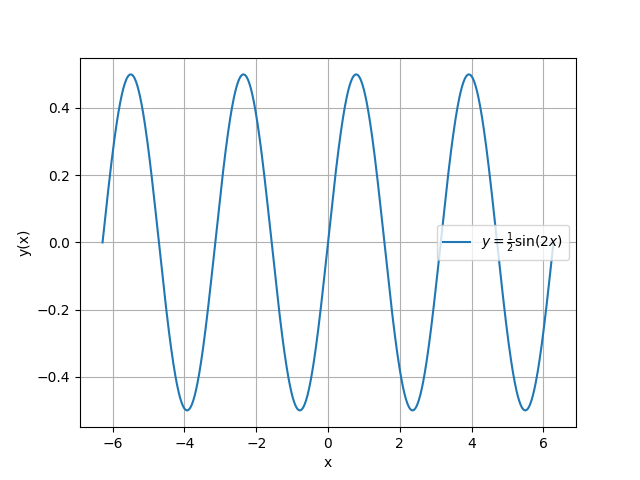
\includegraphics[width=\columnwidth]{2022/ES/36/figs/a.png}
    \caption{$y\brak{x}$ $vs$ $x$ graph}
    \label{figure:gate.2022.es.36Q.1}
\end{figure}

\newpage
\item Let a causal LTI system be governed by the following differential equation, 
\begin{align}
    y\brak{t} + \frac{1}{4}\frac{dy}{dt} = 2x\brak{t} \label{eq1}
\end{align}
where $x\brak{t}$ and $y\brak{t}$ are the input and output respectively. It's impulse response is 
\hfill (GATE EE-2022)\\
\solution
\iffalse
\let\negmedspace\undefined
\let\negthickspace\undefined
\documentclass[journal,12pt,twocolumn]{IEEEtran}
\usepackage{cite}
\usepackage{amsmath,amssymb,amsfonts,amsthm}
\usepackage{algorithmic}
\usepackage{graphicx}
\usepackage{textcomp}
\usepackage{xcolor}
\usepackage{txfonts}
\usepackage{listings}
\usepackage{enumitem}
\usepackage{mathtools}
\usepackage{gensymb}
\usepackage{comment}
\usepackage[breaklinks=true]{hyperref}
\usepackage{tkz-euclide} 
\usepackage{listings}
\usepackage{gvv}                                        
\def\inputGnumericTable{}                                 
\usepackage[latin1]{inputenc}                                
\usepackage{color}                                            
\newtheorem{theorem}{Theorem}[section]
\usepackage{array}                                            
\usepackage{longtable}                                       
\usepackage{calc}                                             
\usepackage{multirow}                                         
\usepackage{hhline}                                           
\usepackage{ifthen}                                           
\usepackage{lscape}
\newtheorem{problem}{Problem}
\newtheorem{proposition}{Proposition}[section]
\newtheorem{lemma}{Lemma}[section]
\newtheorem{corollary}[theorem]{Corollary}
\newtheorem{example}{Example}[section]
\newtheorem{definition}[problem]{Definition}
\newcommand{\BEQA}{\begin{eqnarray}}
\newcommand{\EEQA}{\end{eqnarray}}
\newcommand{\define}{\stackrel{\triangle}{=}}
\theoremstyle{remark}
\newtheorem{rem}{Remark}
\begin{document}
\bibliographystyle{IEEEtran}
\vspace{3cm}
\title{GATE 22 EE/46}
\author{EE23BTECH11040 - Manoj Kumar Ambatipudi$^{*}$% <-this % stops a space
}
\maketitle
\newpage
\bigskip
\renewcommand{\thefigure}{\theenumi}
\renewcommand{\thetable}{\theenumi}
\textbf{QUESTION:}
Let a causal LTI system be governed by the following differential equation, 
\begin{align}
    y\brak{t} + \frac{1}{4}\frac{dy}{dt} = 2x\brak{t} \label{eq1}
\end{align}
where $x\brak{t}$ and $y\brak{t}$ are the input and output respectively. It's impulse response is 
\hfill (GATE EE-2022)\\
\fi
\textbf{Solution:}

From \eqref{eq1}, corresponding Laplace transform, 
\begin{align}
    Y\brak{s} + \frac{1}{4}\brak{sY\brak{s} - y\brak{0}} = 2X\brak{s}
\end{align}
Since it is causal LTI system, 
\begin{align}
    y\brak{0} &= 0\\
	\implies Y\brak{s} + \frac{1}{4}sY\brak{s} &= 2X\brak{s}\\
    \implies Y\brak{s} &= X\brak{s}\frac{8}{4 + s}\\
    \implies H\brak{s} &= \frac{8}{4 + s}\quad ROC:Re\brak{s} > -4
\end{align}
Taking inverse laplace transform and applying causality conditions 
\begin{align}
    h\brak{t} = 8e^{-4t}u\brak{t}
\end{align}
\begin{figure}[h]
\renewcommand\thefigure{1}
    \centering
    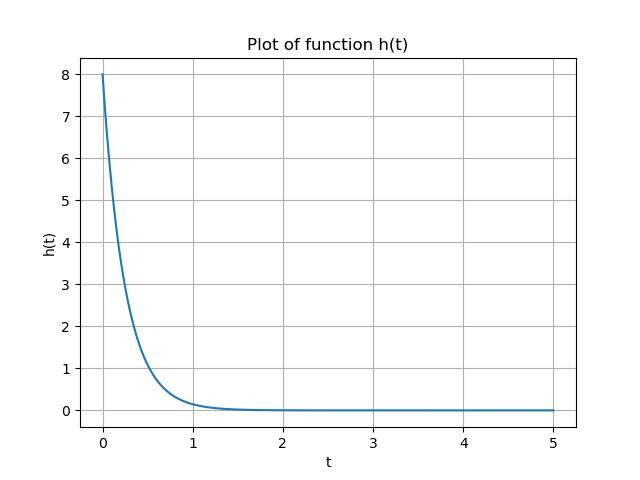
\includegraphics[width=1.0\columnwidth]{2022/EE/46/figs/fig_1.jpg}
    \caption{Plot of $h\brak{n}$, taken from python3}
    \label{fig:enter-label}
\end{figure}


\item Assuming $s>0$; Laplace transform for $f\brak{x} = sin\brak{ax}$ is
\begin{enumerate}[label=(\Alph*)]
    \item $\frac{a}{s^2+a^2}$
    \item $\frac{s}{s^2+a^2}$
    \item $\frac{a}{s^2-a^2}$
    \item $\frac{s}{s^2-a^2}$
\end{enumerate} \hfill(GATE 2022 ES)\\
\solution
\iffalse
\let\negmedspace\undefined
\let\negthickspace\undefined
\documentclass[journal,12pt,twocolumn]{IEEEtran}
\usepackage{cite}
\usepackage{amsmath,amssymb,amsfonts,amsthm}
\usepackage{algorithmic}
\usepackage{graphicx}
\usepackage{textcomp}
\usepackage{xcolor}
\usepackage{txfonts}
\usepackage{listings}
\usepackage{enumitem}
\usepackage{mathtools}
\usepackage{gensymb}
\usepackage{comment}
\usepackage[breaklinks=true]{hyperref}
\usepackage{tkz-euclide} 
\usepackage{listings}
\usepackage{gvv}
\def\inputGnumericTable{}                                 
\usepackage[latin1]{inputenc}                                
\usepackage{color}                                            
\usepackage{array}                                            
\usepackage{longtable}                                       
\usepackage{calc}                                             
\usepackage{multirow}                                         
\usepackage{hhline}                                           
\usepackage{ifthen}                                           
\usepackage{lscape}

\newtheorem{theorem}{Theorem}[section]
\newtheorem{problem}{Problem}
\newtheorem{proposition}{Proposition}[section]
\newtheorem{lemma}{Lemma}[section]
\newtheorem{corollary}[theorem]{Corollary}
\newtheorem{example}{Example}[section]
\newtheorem{definition}[problem]{Definition}
\newcommand{\BEQA}{\begin{eqnarray}}
\newcommand{\EEQA}{\end{eqnarray}}
\newcommand{\define}{\stackrel{\triangle}{=}}
\theoremstyle{remark}
\newtheorem{rem}{Remark}

\begin{document}

\bibliographystyle{IEEEtran}
\vspace{3cm}

\title{GATE ES22 13}
\author{EE23BTECH11043 - BHUVANESH SUNIL NEHETE$^{*}$% <-this % stops a space
}
\maketitle
\newpage
\bigskip

\renewcommand{\thefigure}{\theenumi}
\renewcommand{\thetable}{\theenumi}

\bibliographystyle{IEEEtran}

\textbf{Question:}
Assuming $s>0$; Laplace transform for $f\brak{x} = sin\brak{ax}$ is
\begin{enumerate}[label=(\Alph*)]
    \item $\frac{a}{s^2+a^2}$
    \item $\frac{s}{s^2+a^2}$
    \item $\frac{a}{s^2-a^2}$
    \item $\frac{s}{s^2-a^2}$
\end{enumerate}

\solution
\fi
\begin{align}
\mathcal{L}\brak{f\brak{x}}=\int_{-\infty}^{\infty}e^{-sx}f\brak{x}dx\\
\text{We can write} \quad\sin\brak{ax}=\frac{e^{ax}-e^{-ax}}{2i}\label{13es22eq1}
\end{align}
From \eqref{13es22eq1}
\begin{align}
\mathcal{L}\brak{\sin\brak{ax}}&=\int_{0}^{\infty}e^{-sx}\brak{\frac{e^{iax}-e^{-iax}}{2i}}dx\\
&=\frac{1}{2i}\int_{0}^{\infty}e^{-x\brak{s-ia}}-e^{-x\brak{s+ia}}dx\\
&=\frac{1}{2i}\brak{\frac{e^{-x\brak{s-ia}}}{-\brak{s-ia}}+\frac{e^{-x\brak{s+ia}}}{-\brak{s+ia}}}_{0}^{\infty}\\
&=\frac{1}{2i}\brak{\frac{1}{s-ia}-\frac{1}{s+ia}}\\
&=\frac{a}{s^2+a^2}
\end{align}

So, option \brak{A} is correct.

\newpage

\item The input $x(t)$ to a system is related to its output $y(t)$ as \\ \\
$\dfrac{dy(t)}{dt} + y(t) = 3x(t-3)u(t-3)$\\ \\
Here $u(t)$ represents a unit-step function.\\
The transfer function of this system is 
\begin{enumerate}
\item[(A)] $\frac{e^{-3s}}{s+3}$\\
\item[(B)] $\frac{3e^{-3s}}{s+1}$\\
\item[(C)] $\frac{3e^{-\brak{s/3}}}{s+1}$\\
\item[(D)] $\frac{e^{-\brak{s/3}}}{s+3}$
\end{enumerate}
\hfill{(GATE IN 2022)}\\
\solution
\iffalse
\let\negmedspace\undefined
\let\negthickspace\undefined
\documentclass[journal,12pt,twocolumn]{IEEEtran}
\usepackage{cite}
\usepackage{amsmath,amssymb,amsfonts,amsthm}
\usepackage{algorithmic}
\usepackage{graphicx}
\usepackage{textcomp}
\usepackage{xcolor}
\usepackage{txfonts}
\usepackage{listings}
\usepackage{enumitem}
\usepackage{mathtools}
\usepackage{gensymb}
\usepackage{comment}
\usepackage[breaklinks=true]{hyperref}
\usepackage{tkz-euclide} 
\usepackage{listings}                                   
\def\inputGnumericTable{}                                 
\usepackage[latin1]{inputenc}                                
\usepackage{color}                                            
\usepackage{array}                                            
\usepackage{longtable}                                       
\usepackage{calc}  
\usepackage{circuitikz}                                           
\usepackage{multirow}                                         
\usepackage{hhline}                                           
\usepackage{ifthen}                                           
\usepackage{lscape}
\newtheorem{theorem}{Theorem}[section]
\newtheorem{problem}{Problem}
\newtheorem{proposition}{Proposition}[section]
\newtheorem{lemma}{Lemma}[section]
\newtheorem{corollary}[theorem]{Corollary}
\newtheorem{example}{Example}[section]
\newtheorem{definition}[problem]{Definition}
\newcommand{\BEQA}{\begin{eqnarray}}
\newcommand{\EEQA}{\end{eqnarray}}
\newcommand{\define}{\stackrel{\triangle}{=}}
\newcommand{\brak}[1]{\langle #1 \rangle}
\theoremstyle{remark}
\newtheorem{rem}{Remark}

\begin{document}
\bibliographystyle{IEEEtran}
\vspace{3cm}
\title{\textbf{GATE 2022 EE}}
\author{EE23BTECH11023-ABHIGNYA GOGULA}
\maketitle
\newpage
\bigskip
\renewcommand{\thefigure}{\theenumi}
\renewcommand{\thetable}{\theenumi}
\textbf{Question27:}
\\An inductor having a $Q$-factor of 60 is connected in series with a capacitor having a $Q$-factor of 240. The overall $Q$-factor of the circuit is \_\_\_\_\_\_\_\_\_\_. (Round off to the nearest integer) \\
\hfill Gate 2022 EE Question 27\\
\section*{Solution}
\fi
\begin{circuitikz}
    \draw (0,0) to[R, l=$R_1$] (2,0) to[L, l=$L$] (4,0);
\end{circuitikz}
\begin{align}
Q_1=\frac{\omega_0 L}{R_1}
\end{align}
\begin{circuitikz}
    \draw (0,0) to[R, l=$R_2$] (2,0) to[C, l=$C$] (4,0);
\end{circuitikz}
\begin{align}
Q_2=\frac{1}{\omega_0 C R_2}
\end{align}
at resonance as $\omega_0 L =\frac{1}{\omega_0 C}$ hence
\begin{align}
Q_2=\frac{\omega_0 L}{R_2}
\end{align}
\begin{circuitikz}
    \draw (0,0) to[R, l=$R_1$] (2,0) to[L, l=$L$] (4,0) to[R, l=$R_2$] (6,0) to[C, l=$C$] (8,0);
\end{circuitikz}
\begin{align}
Q = \frac{\omega_0 L}{R_1+R_2}\\
Q = \frac{1}{\frac{R_1}{\omega_0 L}+\frac{R_2}{\omega_0 L}}
\end{align}
\begin{equation}
Q =\frac{Q_1 Q_2}{Q_1+Q_2}
\label{eq:EE 27eq1}
\end{equation}
then from \eqref{eq:EE 27eq1}
\begin{align}
Q=\frac{60 \times 240}{60+240}\\
Q=48
\end{align}
%\end{document}

\newpage
\pagebreak
\item Let $x_1\brak{t} = e^{-t}u\brak{t}$ and $x_2\brak{t} =u\brak{t}-u\brak{t-2}$, where $u\brak{.}$ denotes the unit step function. If $y\brak{t}$ denotes the convolution of $x_1\brak{t}$ and $x_2\brak{t}$ ,then $\lim\limits_{t \to \infty} y\brak{t}$ = \underline{\hspace{1cm}}. (Rounded off to one decimal place)\\
\hfill(GATE EC 2022 )\\
\solution
\iffalse
\documentclass[journal,12pt,onecolumn]{IEEEtran}
\usepackage{cite}
\usepackage{amsmath,amssymb,amsfonts,amsthm}
\usepackage{algorithmic}
\usepackage{graphicx}
\usepackage{textcomp}
\usepackage{xcolor}
\usepackage{txfonts}
\usepackage{listings}
\usepackage{enumitem}
\usepackage{mathtools}
\usepackage{gensymb}
\usepackage{comment}
\usepackage[breaklinks=true]{hyperref}
\usepackage{tkz-euclide}
\usepackage{listings}
\usepackage{gvv}
\def\inputGnumericTable{}
\usepackage[latin1]{inputenc}
\usepackage{color}
\usepackage{array}
\usepackage{longtable}
\usepackage{calc}
\usepackage{multirow}
\usepackage{hhline}
\usepackage{ifthen}
\usepackage{lscape}

\newtheorem{theorem}{Theorem}[section]
\newtheorem{problem}{Problem}
\newtheorem{proposition}{Proposition}[section]
\newtheorem{lemma}{Lemma}[section]
\newtheorem{corollary}[theorem]{Corollary}
\newtheorem{example}{Example}[section]
\newtheorem{definition}[problem]{Definition}
\newcommand{\BEQA}{\begin{eqnarray}}
    \newcommand{\EEQA}{\end{eqnarray}}
\newcommand{\define}{\stackrel{\triangle}{=}}
\theoremstyle{remark}
\newtheorem{rem}{Remark}

\begin{document}
    
    \bibliographystyle{IEEEtran}
    \vspace{3cm}
    
    \title{Gate 2021 BM Q8}
    \author{EE23BTECH11212 - Manugunta Meghana Sai$^{*}$% <-this % stops a space
    }
    \maketitle
    \bigskip
    
    \renewcommand{\thefigure}{\theenumi}
    \renewcommand{\thetable}{\theenumi}
    
    \vspace{3cm}
    
    For a linear stable second order system, if the unit step response is such that peak time is twice the rise time, then the system is . 
    \begin{enumerate}
    \item underdamped\\
    \item undamped\\
    \item overdamped\\
    \item critically damped\\
    \end{enumerate}
    \solution
    \fi
    \begin{table}[h!]
 	\centering
 	\resizebox{6 cm}{!}{
 		\begin{tabular}{|c|c|c|}
	\hline
	\textbf{Parameter} &  \textbf{Description}\\[6pt]
	\hline
	$\omega_{n}$ & natural frequency\\[6pt]
	\hline
	$\zeta$ & damping ratio \\[6pt]
	\hline 
	$\theta$ & is the angle in the complex plane corresponding to the pole location\\[6pt]
	\hline
\end{tabular}

 	}
 	\caption{Given Parameters}
 	\label{tab:msmBMgate8tab1}
     \end{table} 
    \\The rise time is given by:
    \begin{align}
    t_{r} = \frac{\pi-\theta}{\omega_{n} \sqrt{1-\zeta^{2}}}
    \end{align}
    The peak time is given by:
    \begin{align}
    t_{p} = \frac{\pi}{\omega_{n} \sqrt{1-\zeta^{2}}}
    \end{align}
    as, peak time is twice the rise time:
    \begin{align}
    t_{p} &= 2t_{r}\\
    \frac{\pi}{\omega_{n} \sqrt{1-\zeta^{2}}} &= 2\frac{\pi-\theta}{\omega_{n} \sqrt{1-\zeta^{2}}}\\
    \theta &= \frac{\pi}{2}
    \end{align}
    as, $\theta = \frac{\pi}{2}$, both roots of the system are imaginary, so 
    \begin{align}
    G\brak{s} = \frac{\omega_n^2}{s^2 + 2\zeta\omega_n s + \omega_n^2}
    \end{align}
    So, for the denominator to have two imaginary roots
    \begin{align}
      s = +\j\omega_{n}\\
      s = -\j\omega_{n}
    \end{align}
     $2\zeta\omega_n$ should be zero.
   
    \begin{align}
    \zeta = 0
    \end{align}
    The Routh-Hurwitz criterion is a method used to determine the stability of a system based on the locations of the roots of the characteristic equation in the complex plane.\\
    
     The coefficients of $s$, $s^{2}$ and 1, which are $2\zeta \omega_{n}$, $1$ and $\omega_{n}^{2}$ are non negative, hence the system is stable.So,the syatem is either undamped or overdamped.As, 
    $\zeta$ is zero, system is undamped. 
%\end{document}

\newpage

\item A unity-gain negative-feedback control system has a loop-gain $L\brak{s}$ given by
\begin{align}
    L\brak{s} = \frac{6}{s\brak{s-5}}
\end{align}
The closed loop system is \rule{1cm}{0.15mm}
\begin{enumerate}
    \item Causal and stable
    \item Causal and unstable
    \item Non-causal and stable
    \item Non-causal and unstable
\end{enumerate}
\hfill(GATE IN 2022)\\
\solution
\iffalse
\let\negmedspace\undefined
\let\negthickspace\undefined
\documentclass[journal,12pt,twocolumn]{IEEEtran}
\usepackage{cite}
\usepackage{amsmath,amssymb,amsfonts,amsthm}
\usepackage{algorithmic}
\usepackage{graphicx}
\usepackage{textcomp}
\usepackage{xcolor}
\usepackage{txfonts}
\usepackage{listings}
\usepackage{enumitem}
\usepackage{mathtools}
\usepackage{gensymb}
\usepackage{comment}
\usepackage[breaklinks=true]{hyperref}
\usepackage{tkz-euclide} 
\usepackage{listings}
\usepackage{gvv}                                        
\def\inputGnumericTable{}                                 
\usepackage[latin1]{inputenc}                                
\usepackage{color}                                            
\usepackage{array}                                            
\usepackage{longtable}                                       
\usepackage{calc}                                             
\usepackage{multirow}                                         
\usepackage{hhline}                                           
\usepackage{ifthen}                                           
\usepackage{lscape}
\usepackage{placeins}
\usepackage{xparse}


\newtheorem{theorem}{Theorem}[section]
\newtheorem{problem}{Problem}
\newtheorem{proposition}{Proposition}[section]
\newtheorem{lemma}{Lemma}[section]
\newtheorem{corollary}[theorem]{Corollary}
\newtheorem{example}{Example}[section]
\newtheorem{definition}[problem]{Definition}
\newcommand{\BEQA}{\begin{eqnarray}}
\newcommand{\EEQA}{\end{eqnarray}}
\newcommand{\define}{\stackrel{\triangle}{=}}
\theoremstyle{remark}
\newtheorem{rem}{Remark}

\graphicspath{ {./figs/} } 

\begin{document}

\bibliographystyle{IEEEtran}
\vspace{3cm}

\Large\title{GATE 2022 IN 15}
\large\author{EE23BTECH11032 - Kaustubh Parag Khachane $^{*}$% <-this % stops a space
}
\maketitle
\newpage
\bigskip

\renewcommand{\thefigure}{\theenumi}
\renewcommand{\thetable}{\theenumi}
\large\textbf{Question GATE 22 IN 15} :\\
A unity-gain negative-feedback control system has a loop-gain $L\brak{s}$ given by
\begin{align}
    L\brak{s} = \frac{6}{s\brak{s-5}}
\end{align}
The closed loop system is \rule{1cm}{0.15mm}
\begin{enumerate}
    \item Causal and stable
    \item Causal and unstable
    \item Non-causal and stable
    \item Non-causal and unstable
\end{enumerate}
\hfill(GATE IN 2022)\\
\solution\\
\fi
\begin{table}[!ht] 
\centering
\setlength{\extrarowheight}{8pt}
\begin{tabular}{|l|l|l|}
    \hline
    \textbf{Parameter} & \textbf{Description} & \textbf{Value} \\
    \hline
     $L\brak{s}$ & Forward loop transfer function & $\frac{6}{s\brak{s-5}}$ \\\hline
     $H\brak{s}$ & Feedback path transferfunction & 1 \\\hline
     $T\brak{s}$ & Transfer function & $\frac{L\brak{s}}{1 + L\brak{s}H\brak{s}}$ \\\hline
    \end{tabular}
  \vspace{4mm}
 \caption{Parameter Table}
 \label{tab:table0_in15}
\end{table}

From \tabref{tab:table0_in15}, the transfer function of the system is given by,
\begin{align}
    T\brak{s} &= \frac{\frac{6}{s\brak{s-5}}}{1 + 1\frac{6}{s\brak{s-5}}}\\
    &= \frac{6}{s^2 - 5s + 6}
\end{align}
The poles of the system are given by the roots of the denominator of transfer function,
\begin{align}
    s^2 - 5s + 6 = 0
\end{align}
$\therefore$ The poles of the system are $s = 2$ and $s = 3$.\\
As the poles are positive, the output will increase without bound, causing the system to be unstable.
\\The transfer function of the system is ,
\begin{align}
    T\brak{s} = \frac{6}{\brak{s-2}\brak{s-3}}
\end{align}
Clearly, it is dependent only on the past values. Hence, the system is causal.
\\Thus the correct option is B. The system is causal and unstable.
\begin{figure}[!ht]
\centering
\begin{center}
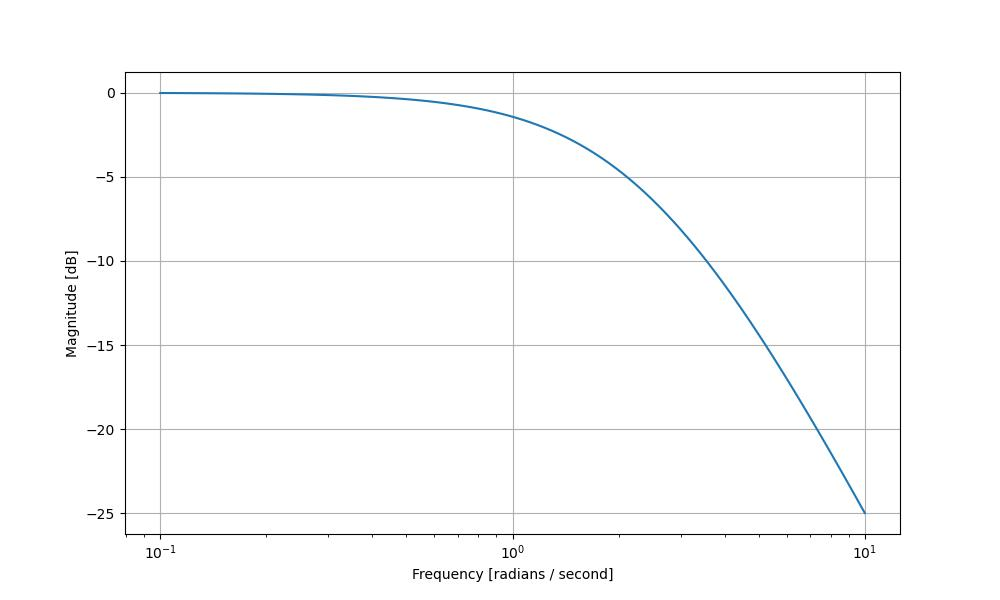
\includegraphics[width=\columnwidth]{2022/IN/15/figs/Figure_1.jpg}
\end{center}
\caption{Magnitude plot for the transfer function}
\end{figure}
\begin{figure}[!ht]
\centering
\begin{center}
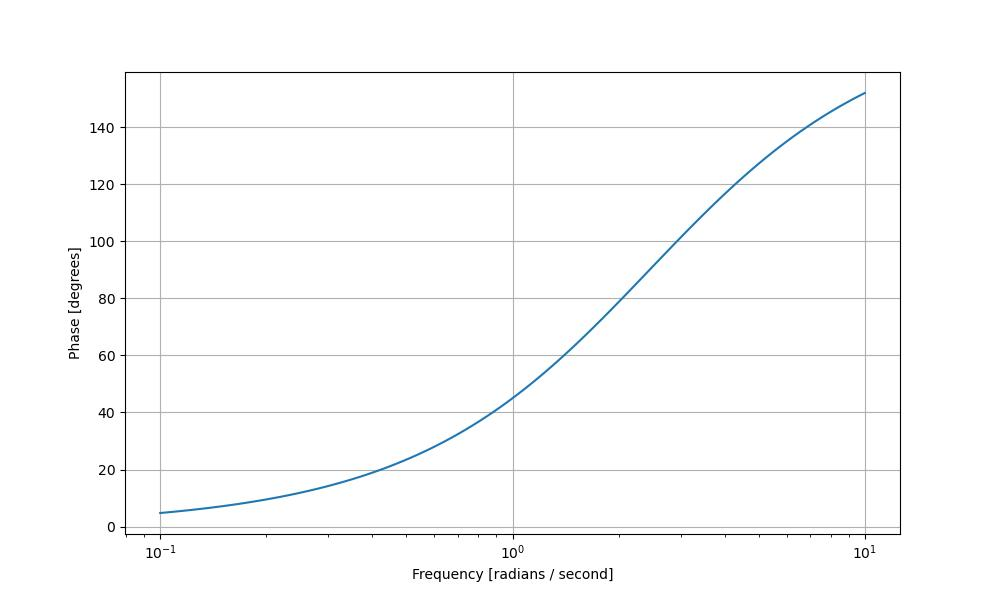
\includegraphics[width=\columnwidth]{2022/IN/15/figs/Figure_2.jpg}
\end{center}
\caption{Phase plot for the transfer function}
\end{figure}

\newpage 
\item Solution of the differential equation $\frac{dy}{dx}-y=cos\brak{x}$ is\\
\begin{align}
\brak{A}\quad y&=\frac{sin\brak{x}-cos\brak{x}}{2}+ce^x\\
\brak{B}\quad y&=\frac{sin\brak{x}+cos\brak{x}}{2}+ce^x\\
\brak{C}\quad y&=\frac{sin\brak{x}+cos\brak{x}}{2}+ce^{-x}\\
\brak{D}\quad y&=\frac{sin\brak{x}-cos\brak{x}}{2}+ce^{-x}
\end{align}
\hfill{GATE BM 2022}\\
\solution
\iffalse
\let\negmedspace\undefined
\let\negthickspace\undefined
\documentclass[journal,12pt,twocolumn]{IEEEtran}
\usepackage{cite}
\usepackage{amsmath,amssymb,amsfonts,amsthm}
\usepackage{algorithmic}
\usepackage{graphicx}
\usepackage{textcomp}
\usepackage{xcolor}
\usepackage{txfonts}
\usepackage{listings}
\usepackage{enumitem}
\usepackage{mathtools}
\usepackage{gensymb}
\usepackage{comment}
\usepackage[breaklinks=true]{hyperref}
\usepackage{tkz-euclide} 
\usepackage{listings}
\usepackage{gvv}                                        
\def\inputGnumericTable{}                                 
\usepackage[latin1]{inputenc}                                
\usepackage{color}                                            
\usepackage{array}                                            
\usepackage{longtable}                                       
\usepackage{calc}                                             
\usepackage{multirow}                                         
\usepackage{hhline}                                           
\usepackage{ifthen}                                           
\usepackage{lscape}

\newtheorem{theorem}{Theorem}[section]
\newtheorem{problem}{Problem}
\newtheorem{proposition}{Proposition}[section]
\newtheorem{lemma}{Lemma}[section]
\newtheorem{corollary}[theorem]{Corollary}
\newtheorem{example}{Example}[section]
\newtheorem{definition}[problem]{Definition}
\newcommand{\BEQA}{\begin{eqnarray}}
\newcommand{\EEQA}{\end{eqnarray}}
\newcommand{\define}{\stackrel{\triangle}{=}}
\theoremstyle{remark}
\newtheorem{rem}{Remark}
\usepackage{circuitikz}
\begin{document}

\bibliographystyle{IEEEtran}
\vspace{3cm}

\title{GATE-2022, BM-37}
\author{EE23BTECH11033- JASWANTH KILLANA}
\maketitle
\newpage
\bigskip

\renewcommand{\thefigure}{\theenumi}
\renewcommand{\thetable}{\theenumi}
Question: Solution of the differential equation $\frac{dy}{dx}-y=cos\brak{x}$ is
\begin{align}
\brak{A}\quad y&=\frac{sin\brak{x}-cos\brak{x}}{2}+ce^x\\
\brak{B}\quad y&=\frac{sin\brak{x}+cos\brak{x}}{2}+ce^x\\
\brak{C}\quad y&=\frac{sin\brak{x}+cos\brak{x}}{2}+ce^{-x}\\
\brak{D}\quad y&=\frac{sin\brak{x}-cos\brak{x}}{2}+ce^{-x}
\end{align}
Solution:
\fi
\begin{align}
\frac{dy}{dx}-y&=cos\brak{x}
\end{align}
Apply laplace transform
\begin{align}
\mathcal{L}\brak{\frac{dy}{dx}}-\mathcal{L}\brak{y}&=\mathcal{L}\brak{{cos\brak{x}}}
\end{align}
\begin{table}[!ht]
 \centering
  \begin{tabular}{|c|c|c|}
\hline
\textbf{parameter}& \textbf{laplace transform }
\\\hline
\multirow{3}{1em}\\$\frac{dy}{dx}$&$sY\brak{s}-y\brak{0}$
\\\hline
$y$&$Y\brak{s}$
\\\hline
$cos\brak{x}$&$\frac{s}{s^{2}+1}$
\\\hline
$sin\brak{x}$&$\frac{1}{s^{2}+1}$
\\\hline
$e^x$&$\frac{1}{s-1}$
\\\hline
\end{tabular}



   \caption{transformation}
   \end{table}
\begin{align}
\implies sY\brak{s}-y\brak{0}-Y\brak{s}&=\frac{s}{s^{2}+1}\\
Y\brak{s}\brak{s-1}&=y\brak{0}+\frac{s}{s^{2}+1}\\
Y\brak{s}&=\frac{s+y\brak{0}\brak{s^{2}+1}}{\brak{s-1}\brak{s^{2}+1}}\\
Y\brak{s}&=\frac{A}{s-1}+\frac{Bs+C}{s^2+1}\\
A&=y\brak{0},B=\frac{-1}{2},c=\frac{1}{2}\\
\implies Y\brak{s}&=\frac{y\brak{0}}{s-1}+\frac{-s+1}{2\brak{s^2+1}}
\end{align}
apply inverse laplace transform
\begin{align}
\mathcal{L^-}\brak{Y\brak{s}}&=\mathcal{L^-}\brak{\frac{y\brak{0}}{s-1}}+\mathcal{L^-}\brak{\frac{-s+1}{2\brak{s^2+1}}}\\
y\brak{x}&=y\brak{0}e^x+\frac{sin\brak{x}-cos\brak{x}}{2}
\end{align} 
\begin{align}
 y\brak{0}&=c
 \end{align}
 As both are constants
 \begin{align}
 \implies y&=\frac{sin\brak{x}-cos\brak{x}}{2}+ce^x
\end{align}
Option A is correct
%\end{document}

\newpage

\end{enumerate}
